%!TEX root = thesis.tex"`

\chapter{Идеальный ферми--газ}
\acrfull{ifg} -- это система невзаимодействующих фермионов (частиц, имеющих полуцелый спин).
Согласно принципу запрета Паули \cite{Pauli:ZP:1925,Pauli:PR:1940}, в заданном квантовом состоянии может находиться только один фермион.
Это приводит приводит к нескольким следствиям.
Во-первых, полная энергия \acrshort{ifg} при нулевой температуре отлична от нуля.
Во-вторых, давление \acrshort{ifg} не равно нулю при нулевой температуре, в отличие от идеального больцмановского газа.

В дальнейшей части работы, если не оговорено иное, используется атомная система единиц, в которой редуцированная постоянная Планка, масса и заряд фермиона равны единице.
Помимо этого, постоянная Больцмана тоже положена равной единице.

\section{Химический потенциал и его производные}
Для системы фермионов распределение частиц по энергиям задается статистикой Ферми--Дирака \cite{Landau:statmech:1958}:
\begin{equation}
    n_k = \frac{1}{\exp{[(\varepsilon_k - \mu)/T]} + 1}.
    \label{eq:fd}
\end{equation}
Здесь $\mu$ есть химический потенциал, $T$ -- температура системы, а $\epsilon_k$ -- энергия $k$-ого квантового состояния.
Полное число частиц получается суммированием \eqref{eq:fd} по всем возможным значениям энергии.
Полагая $\epsilon_k = p^2_{k} / (2m)$ и переходя к квазинепрерывному спектру по $k$, после сведения к интегрированию по энергии получим:
\begin{equation}
    \label{eq:conc}
    \frac{N}{V}=\frac{g}{\sqrt{2} \pi^{2}} \int_{0}^{\infty} \frac{\sqrt{\varepsilon} d \varepsilon}{e^{(\varepsilon-\mu) / T}+1}.
\end{equation}
Здесь $V$~--- объем системы, $g$~--- фактор вырождения по спину (для электрона $g = 2$).
Вводя безразмерный химический потенциал $y = \mu / T$ и объем, приходящийся на одну частицу $v = V / N$, можно переписать \eqref{eq:conc} в следующем виде:
\begin{equation}
    \frac{1}{v} = \frac{g T^{3/2}}{\sqrt{2}\pi^2}I_{1/2}(y).
    \label{eq:mu_equation}
\end{equation}
Здесь введен так называемый \gls{fdi}:
\begin{equation}
    \label{eq:fermi-dirak_integral_definition}
    I_{j}(y)= \int_{0}^{\infty} \frac{t^{j}}{e^{t-y}+1} dt,
\end{equation}
обладающий следующим важным свойством при дифференцировании по параметру:
\begin{equation}
    \label{eq:ifg_diff_rule}
    \frac{d}{dx}\, I_k (x) = k I _{k-1} (x)
\end{equation}

Уравнение \eqref{eq:mu_equation} задает химический потенциал как функцию от температуры и удельного объема: $\mu = \mu(v, T)$.
В разделах \ref{sec:asymp_low}, \ref{sec:asymp_high} приводится его решение в пределе низких и высоких температур.

В дальнейшем нам понадобятся первые и вторые производные $\mu(v, T)$.
Для их получения продифференцируем \eqref{eq:mu_equation} по соответствующим переменным с учетом свойства \eqref{eq:ifg_diff_rule} и разрешим получающиеся уравнения относительно производных. Это даст следующие результаты:
\begin{equation}
   \label{eq:mu_T}
   y'_{T} = -\frac{3 I_{1 / 2}(y)}{T I_{-1 / 2}(y)}
\end{equation}

\begin{equation}
   \label{eq:mu_v}
   y'_{v} = - \frac{2 I_{1 / 2} (y)}{v I_{-1 / 2} (y)}\,
\end{equation}

\begin{equation}
   \label{eq:mu_vv}
   y''_{vv} = \frac{4 I_{1 / 2} (y)}{v^2 I_{-1 / 2} (y)}\, + \frac{2 I_{-3 /2} (y) I_{1 / 2} ^2 (y)}{v^2 I_{-1 /2}^3 (y)}\,
\end{equation}

\begin{equation}
   \label{eq:mu_TT}
   y''_{TT} = \frac{15 I_{1 /2} (y)}{2 T^2 I_{-1 /2} (y)}\, + \frac{9 I_{-3 /2}(y) I_{1 /2}^2 (y)}{2 T^2 I_{-1 /2}^3 (y)}\,
\end{equation}

\begin{equation}
   \label{eq:mu_vT}
   y''_{vT} = y''_{Tv} = \frac{3 I_{1 /2}(y)}{T v I_{-1 /2} (y)}\, + \frac{3 I_{-3 /2} (y) I_{1 /2}^2 (y)}{T v I_{-1 /2}^3 (y)}\,
\end{equation}

\section{Термодинамические функции \texorpdfstring{\acrshort{ifg}}{ИФГ}}
Согласно \cite{kirzhnits:UFN:1975}, выражение для свободной энергии Гельмгольца \acrshort{ifg} имеет вид:
\begin{equation}
   \label{eq:helmholtz_potential}
   F = \frac{g}{\sqrt{2}\pi^2}\,  T^{5 / 2} v \left( y \, I_{1 /2} (y) - \frac{2}{3}\, I_{3 / 2} (y) \right)
   = T\left[y - \frac{2}{3}\frac{I_{3/2}(y)}{I_{1/2}(y)}\right].
\end{equation}
Последнее равенство получается подстановкой $v$ из \eqref{eq:mu_equation}.
Из выражения для $F$ можно получить остальные термодинамические величины:
\begin{equation}
    \label{eq:PES}
    P = -F'_v;\quad
    E = F - TF'_T;\quad
    S = -F'_T;
\end{equation}
\begin{equation}
    \label{eq:CVCP}
    C_V = -TF''_{TT};\quad
    C_P = -TF''_{TT} + \frac{T(F''_{vT})^2}{F''_{vv}};
\end{equation}
\begin{equation}
    \label{eq:CTCS}
    C_T^2 = v^2F''_{vv};\quad
    C_S^2 = v^2F''_{vv} - \frac{v^2(F''_{vT})^2}{F''_{TT}};\quad
    \gamma = \frac{VF''_{vT}}{TF''_{TT}};\ \ldots
\end{equation}
Здесь $P$ -- давление, $C_V$ и $C_P$ -- теплоемкости при постоянном объеме и давлении, соответственно, $C_T$ и $C_S$ -- изотермическая и адиабатическая скорости звука, $\gamma$ -- параметр Грюнайзена.

Используя формулы \eqref{eq:mu_T} -- \eqref{eq:mu_vT}, получим для термодинамических функций \acrshort{ifg}:
\begin{equation}
   \label{eq:pressure}
   P = \frac{g \sqrt{2} T^{5 /2} I_{3 / 2}(y)}{3 \pi^{2}}
   = \frac{2T}{3v}\frac{I_{3/2}(y)}{I_{1/2}(y)},
\end{equation}

\begin{equation}
   \label{eq:energy}
   E = \frac{g v}{\sqrt{2}\pi^2} T^{5 /2} I_{3 / 2}(y)
   = \frac{I_{3/2}(y)}{I_{1/2}(y)}T,
\end{equation}

\begin{equation}
   \label{eq:entropy}
   S = -\frac{g\sqrt{2} T^{3 /2} v\left(3 I_{1 / 2}(y) y-5 I_{3 / 2}(y)\right)}{6 \pi^{2}}
   = -\frac{3I_{1/2}(y) - 5I_{3/2}(y)}{3I_{1/2}(y)},
\end{equation}

\begin{equation}
   \label{eq:C_v}
   C_v = \frac{g\sqrt{2} T^{3 /2} v \left( 5 I_{-1 / 2 } (y) I_{3 /2} (y) - 9 I_{1 / 2}^2 (y)\right)}{4\pi^2 I_{-1 / 2} (y)}
   = \frac{5}{2}\,\frac{I_{3/2}(y)}{I_{1/2}(y)} - \frac{9}{2}\,\frac{I_{1/2}(y)}{I_{-1/2}(y)},
\end{equation}

\begin{multline}
   \label{eq:C_P}
      C_{P} = \frac{5 g \sqrt{2} T^{3 / 2} v\left(5 I_{-1 / 2}(y) I_{3 / 2}(y)-9 I_{1 / 2}^{2}(y)\right) I_{3 / 2}(y)}{36 \pi^{2} I_{1 / 2}^{2}(y)}
      = {}\\
      \frac{25}{18}\,\frac{I^2_{3/2}(y)I_{-1/2}(y)}{I^3_{1/2}(y)} - \frac{5}{2}\,\frac{I_{3/2}(y)}{I_{1/2}(y)},
\end{multline}

\begin{equation}
   \label{eq:C_T}
   C_{T}^2 = \cfrac{\sqrt{2}g}{\pi^2}\,  \cfrac{T^{5 /2} v I_{1 / 2}^2 (y)}{I_{-1 / 2} (y)}
   = \frac{2TI_{1/2}(y)}{I_{-1/2}(y)},
\end{equation}

\begin{equation}
   \label{eq:C_S}
   C_{S}^2 = \cfrac{5 \sqrt{2}g}{9 \pi^2}\, T^{5 / 2} v I_{3 / 2} (y)
   = \frac{10T I_{3/2}(y)}{9I_{1/2}(y)}.
\end{equation}

В разделах \ref{sec:asymp_low} и \ref{sec:asymp_high} обсуждается асимптотическое поведение данных величин в пределе низких и высоких температур.

\section{Асимптотики при низких температурах}
\label{sec:asymp_low}
При низких температурах выполняется условие $y = \mu / T \gg 1$.
В этом пределе справедливо разложение \cite{Shemyakin:JPA:2010}:
\begin{equation}
    \label{eq:Ihalf}
    I_{1/2}(y) \approx
    \frac{2y^{3/2}}{3}\left[1+\frac{\pi^2}{8y^2}+\frac{7\pi^4}{640y^4} + \ldots\right],
\end{equation}
\begin{equation}
    \label{eq:I3half}
    I_{3/2}(y) \approx \frac{2y^{5/2}}{5}\left[1+\frac{5\pi^2}{8y^2}-\frac{7\pi^4}{384y^4} + \ldots\right].
\end{equation}
Если оставить только первый член в \eqref{eq:Ihalf}, то выражение \eqref{eq:mu_equation} станет независимым от температуры.
Это соответствует случаю $T=0$, в котором химический потенциал равен энергии Ферми:
\begin{equation}
    \mu|_{T = 0} = \varepsilon_F = \left( \frac{3\pi^2}{\sqrt{2}gv} \right)^{2/3}.
\end{equation}
Если же оставить первые два члена в \eqref{eq:Ihalf} и подставить $y = \epsilon_F / T$ во второй из них, то можно получить первую поправку для химического потенциала:
\begin{equation}
    \mu \approx \varepsilon_F\left[
    1 - \frac{\pi^2}{12}\left( \frac{T}{\varepsilon_F} \right)^2 \right].
    \label{eq:mulowtemp}
\end{equation}
Подставляя \eqref{eq:Ihalf}, \eqref{eq:I3half} в \eqref{eq:helmholtz_potential} и оставляя первые два члена, получим:
\begin{equation}
    F \approx \frac{g}{\sqrt{2}\pi^2}T^{5/2}v\left[ \frac{2}{5}y^{5/2} - \frac{\pi^2}{12}y^{1/2} \right]
    = \frac{3T^{5/2}}{2\varepsilon_F^{3/2}}\left[ \frac{2}{5}y^{5/2} - \frac{\pi^2}{12}y^{1/2} \right].
    \label{eq:Flowtemp}
\end{equation}
Наконец, подстановка \eqref{eq:mulowtemp} в \eqref{eq:Flowtemp} даст:
\begin{equation}
    \label{eq:F_lt}
    F \approx \frac{3}{5}\epsilon_F\left[ 1 - \frac{5\pi^2}{12}\left( \frac{T}{\epsilon_F} \right)^2 \right]
    = Av^{-2/3} - \frac{\beta}{2}T^2 v^{2/3}.
\end{equation}
Здесь $\beta = (g \pi / 6)^{3 / 2}$~--- так называемый коэффициент электронной теплоемкости \cite{Landau:statmech:1958},
\begin{equation}
    \label{eq:A_def}
    A = \frac{3}{5}\left( \frac{3\pi^2}{\sqrt{2}g} \right)^{2/3}.
\end{equation}

Используя формулы \eqref{eq:PES}, \eqref{eq:CVCP}, \eqref{eq:CTCS}, получим в пределе низких температур:
\begin{equation}
    \label{eq:P_lt}
    P = \frac{2}{3}Av^{-5/3} + \frac{\beta}{3}T^2 v^{-1/3},
\end{equation}
\begin{equation}
    \label{eq:E_lt}
    E = Av^{-2/3} + \frac{\beta}{2}T^2 v^{2/3} = \frac{3}{5}\varepsilon_F + \frac{\beta}{2}T^2 v^{2/3},
\end{equation}
\begin{equation}
    \label{eq:S_lt}
    S = \beta T v^{2/3},
\end{equation}
\begin{equation}
    \label{eq:cv_lt}
    C_v = \beta T v^{2/3},
\end{equation}
\begin{equation}
    \label{eq:cp_lt}
    C_P = \beta T v^{2/3},
\end{equation}
\begin{equation}
    \label{eq:ct2_lt}
    C_T^2 = \frac{10A}{9}v^{-2/3} + \frac{\beta}{9}T^2 v^{2/3},
\end{equation}
\begin{equation}
    \label{eq:cs2_lt}
    C_S^2 = \frac{10A}{9}v^{-2/3} + \frac{5\beta}{9}T^2 v^{2/3}.
\end{equation}

\section{Асимптотики при высоких температурах}
\label{sec:asymp_high}
При высоких температурах реализуется случай $y = \mu / T \ll -1$.
Поскольку на высоких температурах \acrshort{ifg} переходит в идеальный больцмановский газ (\acrshort{ibg}), обсуждаемые свойства \acrshort{ifg} должны стремиться к классическому результату при $T \to \infty$.
Чтобы это показать, необходимо сделать два замечания.

Во-первых, при $y \ll -1$ можно пренебречь единицей в знаменателе \eqref{eq:fermi-dirak_integral_definition} и получить:
\begin{equation}
    \label{eq:ifg_hightemp}
    I_{k}(y)\approx \Gamma(k + 1)e^{y},
\end{equation}
Здесь $\Gamma(x)$ -- гамма-функция.

В частности,
\begin{equation*}
    I_{-1/2}(y)\approx \sqrt{\pi}e^{y};\quad I_{1/2}(y)\approx \frac{\sqrt{\pi}}{2}e^{y};\quad
    I_{3/2}(y)\approx \frac{3\sqrt{\pi}}{4}e^{y}.
\end{equation*}

Во-вторых, правая часть \eqref{eq:mu_equation} должна оставаться конечной при $T \to \infty$.
Поэтому $I _{1 / 2} (y)$ должен стремиться к нулю или, что равносильно, $\mu / T \to -\infty$.
Это означает, что $\mu$ стремится к $-\infty$, причем быстрее, чем $T$ в первой степени.

Подстановка \eqref{eq:ifg_hightemp} в \eqref{eq:mu_equation} приводит к классическому результату для идеального больцмановского газа:
\begin{equation}
    \label{eq:mu_boltzman}
    \mu = \mu_B = T\ln\left[ \frac{1}{gv}\left( \frac{2\pi}{T} \right)^{3/2} \right]
\end{equation}
что, очевидно, удовлетворяет вышеупомянутым требованиям.

Подстановка разложения \eqref{eq:ifg_hightemp} в выражения для энергии Гельмгольца \eqref{eq:helmholtz_potential}, давления \eqref{eq:pressure}, энергии \eqref{eq:energy}, энтропии \eqref{eq:entropy}, теплоемкостей \eqref{eq:C_v}, \eqref{eq:C_P} и скоростей звука \eqref{eq:C_T}, \eqref{eq:C_S} дает:
\begin{equation}
    F\approx (y - 1)T = \mu - T = -T\ln\left[ gev\left( \frac{T}{2\pi} \right)^{3/2} \right],
\end{equation}
\begin{equation}
    P\approx \frac{T}{v},\quad
    E\approx \frac{3}{2}\,T,\quad
    S\approx \frac{5}{2} - y,
\end{equation}
\begin{equation}
    C_{V}\approx \frac{3}{2},\quad
    C_{P}\approx \frac{5}{2},
\end{equation}
\begin{equation}
    C_{T}^2\approx T,\quad
    C_{S}^2\approx \frac{5}{3}\, T.
\end{equation}

Полученные результаты соответствуют идеальному больцмановскому газу. Чтобы получить первую поправку к ним, необходимо более точное разложение \eqref{eq:fermi-dirak_integral_definition}:
\begin{equation}
    \label{eq:ifg_hightemp_precise}
    I_j(y)\approx e^y \Gamma(j + 1) - \frac{e^{2y}}{2^{j+1}}\Gamma(j + 1),
\end{equation}
В частности,
\begin{equation*}
  I_{1/2}(y)\approx \frac{\sqrt{\pi}e^y}{2}\left(
    1 - \frac{1}{2^{3/2}}e^y
  \right),\
  I_{3/2}(y)\approx \frac{3\sqrt{\pi}}{4}\left(
    1 - \frac{1}{2^{5/2}}e^y
  \right).
\end{equation*}

Подставляя \eqref{eq:ifg_hightemp_precise} в уравнение для $\mu$ \eqref{eq:mu_equation} и затем заменяя $y$ на $\epsilon_F / T$ во втором члене, получим:
\begin{equation}
    \label{eq:mu_equation_high_T}
    \frac{1}{gv}\left( \frac{2\pi}{T} \right)^{3/2}
    = \exp\left(\frac{\mu_B}{T}\right)
    = e^y\left( 1 - \frac{\pi^{3/2}}{gvT^{3/2}} \right).
\end{equation}
Второй член в скобках мал по сравнению с единицей, поэтому можно записать:
\begin{equation}
    \label{eq:muhighT}
    e^y \approx e^{\mu_B / T}\left( 1 + \frac{\pi^{3/2}}{gvT^{3/2}} \right),
\end{equation}
С той же точностью:
\begin{equation*}
  y = \frac{\mu_B}{T} + \frac{\pi^{3/2}}{gvT^{3/2}}.
\end{equation*}

Подставим теперь \eqref{eq:ifg_hightemp_precise} в общую формулу для давления \eqref{eq:pressure}, затем заменим $e^{y}$ в соответствии с \eqref{eq:muhighT} и оставим только члены $T$ и $T^{-1 / 2}$
Это даст:
\begin{equation}
    \label{eq:p_ht}
    P \approx \frac{T}{v} + \frac{\pi^{3/2}}{2\sqrt{T}gv^2}.
\end{equation}
Заметим, что знак <<+>> перед вторым членом соответствует отталкиванию фермионов.

Следуя этому алгоритму, можно получить асимптотическое выражение для удельной энергии Гельмгольца (опять же, оставляя только члены с $T$ в степени, большей или равной $-1 / 2$):
\begin{equation}
    \label{eq:FhighT}
    F = \mu - Pv
    = (\mu_B - T) + \frac{\pi^{3/2}}{2gvT^{1/2}}.
\end{equation}

Остальные асимптотические выражения получаются дифференцированием \eqref{eq:FhighT} в соответствии с общими выражениями \eqref{eq:energy}, \eqref{eq:entropy}, \eqref{eq:C_v}, \eqref{eq:C_P}, \eqref{eq:C_T}, \eqref{eq:C_S}:
\begin{equation}
    \label{eq:EShighT}
    E = \frac{3T}{2} + \frac{3\pi^{3/2}}{4\sqrt{T}gv};\quad S
    = \frac{5}{2} - \ln\left[ \frac{1}{gv}\left( \frac{2\pi}{T} \right)^{3/2} \right] + \frac{\pi^{3/2}}{4T^{3/2}gv};
\end{equation}
\begin{equation}
    \label{eq:CVCPhighT}
    C_V = \frac{3}{2} - \frac{3\pi^{3/2}}{8T^{3/2}gv};\quad
    C_P = \frac{5}{2} - \cfrac{15 \pi^{3 / 2}}{8 T^{3 / 2} g v}\, ;
\end{equation}
\begin{equation}
    \label{eq:CTCShighT}
    C_T^2 = T + \frac{\pi^{3/2}}{\sqrt{T}gv};\quad
    C_S^2 = \frac{5 T}{3} + \frac{5 \pi^{3/2}}{6 \sqrt{T}gv} .
\end{equation}
Из полученных выражений видно, что эффекты вырождения приводят к уменьшению теплоемкости и увеличению скорости звука.

\section{Программная реализация модели \texorpdfstring{\acrshort{ifg}}{ИФГ}}
Формулы \eqref{eq:pressure}, \eqref{eq:energy}, \eqref{eq:entropy}, \eqref{eq:C_v}, \eqref{eq:C_P}, \eqref{eq:C_T}, \eqref{eq:C_S} дают возможность напрямую вычислять характеристики \acrshort{ifg} через \gls{fdi} \eqref{eq:fermi-dirak_integral_definition}.
Для языка \gls{python} существует модуль \href{https://pypi.org/project/fdint}{\texttt{fdint}}, осуществляющий эффективный подсчет упомянутого интеграла \cite{fdint}.

Формулы \eqref{eq:entropy}, \eqref{eq:C_v}, \eqref{eq:C_P} содержат операцию вычитания и поэтому их использование в пределах высоких или низких температур будет приводить к большим ошибкам в расчете.
Для решения этой проблемы в упомянутом диапазоне температур применяются асимптотические формулы для расчета соответствующих величин -- \eqref{eq:EShighT}, \eqref{eq:S_lt} для энтропии, \eqref{eq:CVCPhighT}, \eqref{eq:cv_lt}, \eqref{eq:cp_lt} для теплоемкостей.

Расчет свойств был реализован в виде модуля на \gls{python} и выложен на \gls{pypi} под названием \texttt{ifg} \cite{ifgpy}.
Модуль поддерживает расчет химического потенциала $\mu$, энергии $E$, энтропии $S$, теплоемостей $C_v$, $C_P$, а также скоростей звука $C_T$, $C_S$.
Возможно использование как атомной системы единиц, так и СИ.
Расчеты можно выполнять в широком диапазоне температур и объемов.

\begin{figure}[!h]
    % TODO: (a.kozharin) hspace! <- Mon Jun 22 15:42:48 2020
    \hspace{-1cm}
  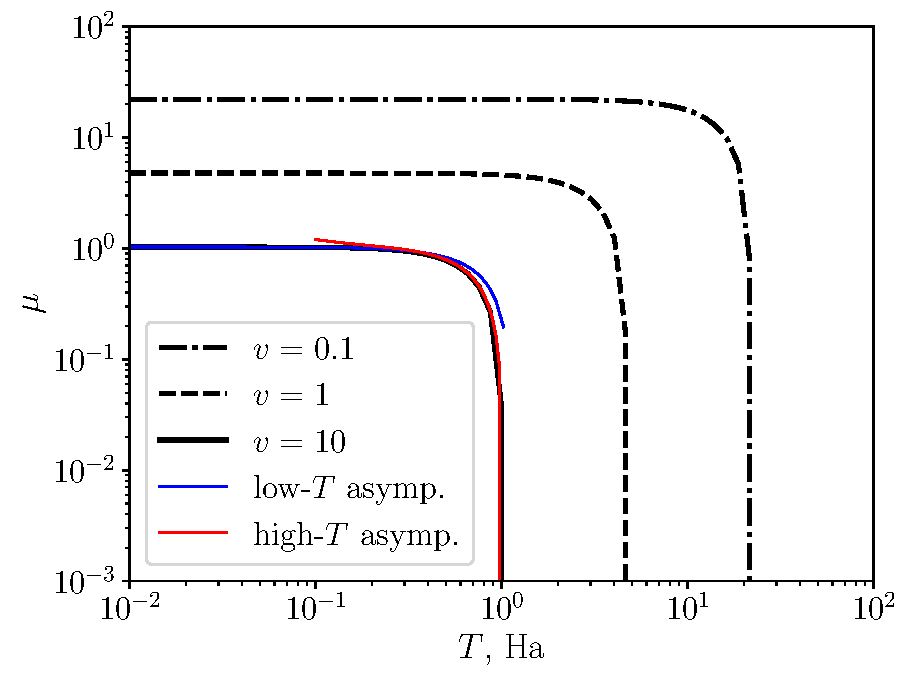
\includegraphics[width=0.5\columnwidth]{img/mu}(a)
  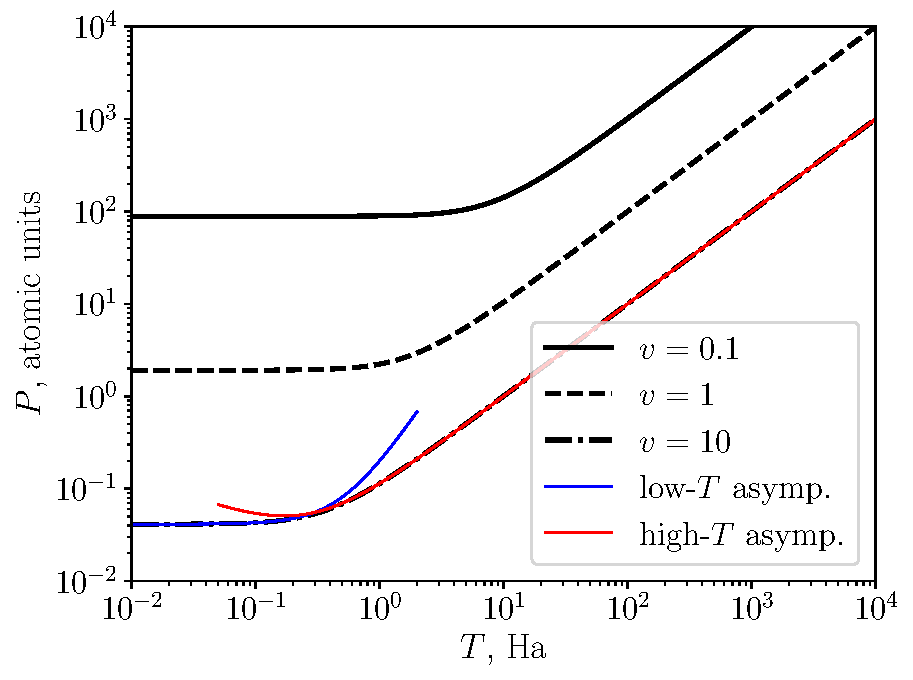
\includegraphics[width=0.5\columnwidth]{img/p}(б)
  \caption{Химический потенциал (a) и давление (б) \acrshort{ifg} при постоянном объеме $v$.}
  \label{fig:chemical_potential}
\end{figure}

\begin{figure}[!h]
    % TODO: (a.kozharin) hspace <- Mon Jun 22 15:43:16 2020
    \hspace{-2cm}
  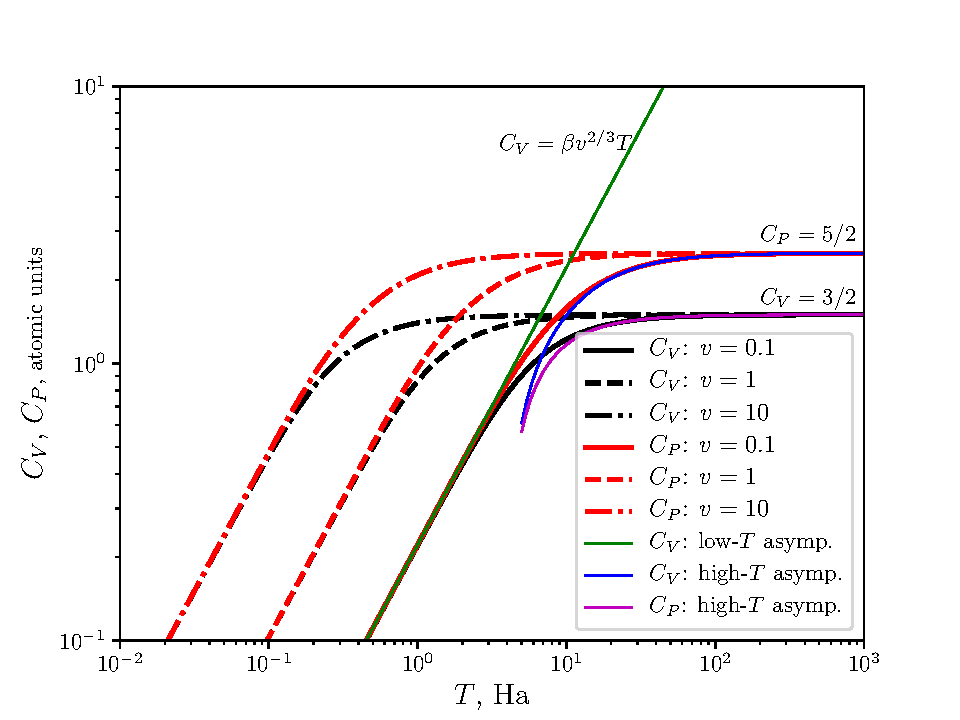
\includegraphics[width=1.2\columnwidth]{img/cv_cp}
  % \caption{Isochoric and isobaric heat capacity of IFG at constant $v$. Red lines---$C_P$, black lines---$C_V$. Solid lines---$v = 0.1$, dashed lines---$v = 1$, dash-dotted lines---$v = 10$. Solid blue line---low-temperature asymptote (\ref{eq:cv_lt}) for $C_V$ and $C_P$ at $v = 0.1$; solid magenta line---high-temperature asymptote (\ref{eq:CVCPhighT}) for $C_V$ at $v = 0.1$; solid organge line---high-temperature asymptote (\ref{eq:CVCPhighT}) for $C_P$ at $v = 0.1$.}
  \caption{Теплоемкости при постоянном объеме и давлении \acrshort{ifg} для фиксированного $v$.}
  \label{fig:heat_capacity}
\end{figure}
\begin{figure}[!h]
    % TODO: (a.kozharin) hspace! <- Mon Jun 22 15:43:30 2020
    \hspace{-1cm}
  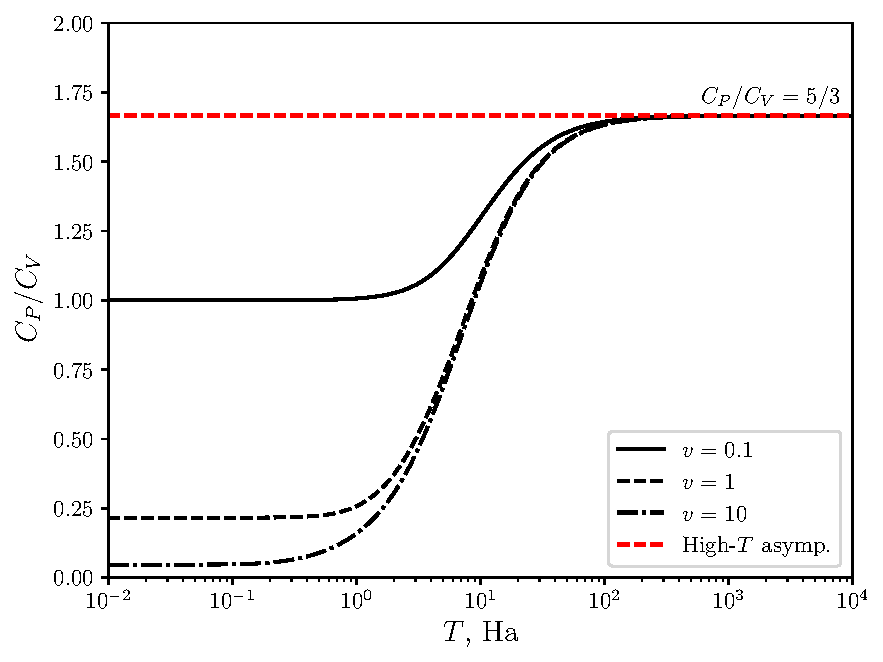
\includegraphics[width=0.5\columnwidth]{img/cp_by_cv}(a)
  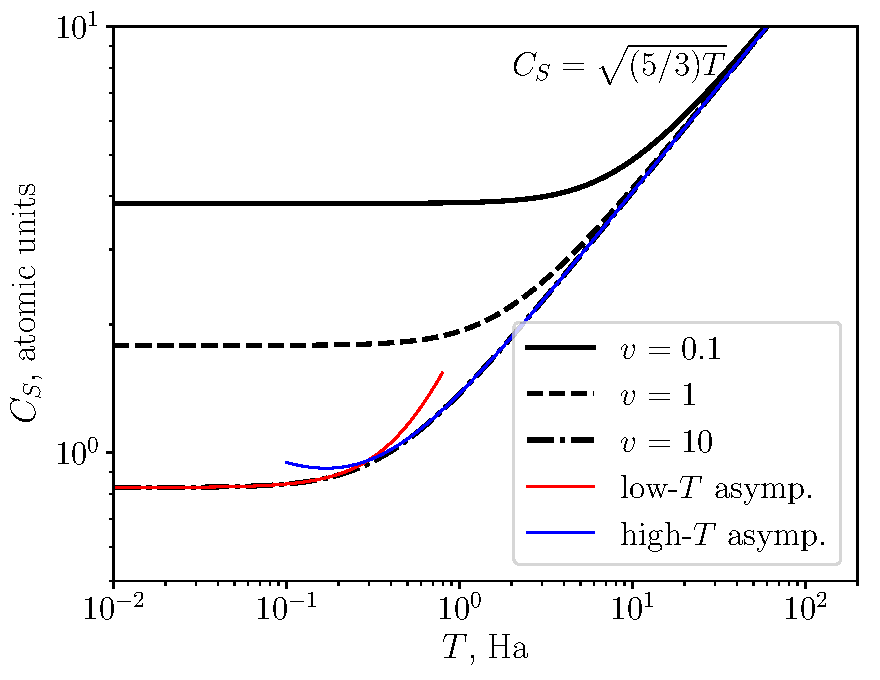
\includegraphics[width=0.5\columnwidth]{img/cs}(б)
  % \caption{Heat capacity ratio (a) and adiabatic sound velocity (b) of IFG at constant $v$. Black lines: solid---$v = 0.1$, dashed---$v = 1$, dash-dotted---$v = 10$. Dashed red line---high-temperature asymptote for $C_P/C_V$; solid blue line---low-temperature asymptote (\ref{eq:cs2_lt}) at $v = 10$; solid red line---high-temperature asymptote (\ref{eq:CTCShighT}) at $v = 10$.}
  \caption{
      Отношение теплоемостей (a) и адиабатическая скорость звука (б) \acrshort{ifg} при постоянном $v$. 
  }
  \label{fig:sound_velocity}
\end{figure}

Из-за упомянутых численных проблемы диапазон допустимого ввода ограничен: $T \in [10^{-49}, 10^{49}]$ для температур и $v \in [10^{-30}, 10^{20}]$ для удельных объемов.
В этих диапазонах гарантируется точность $\delta = 10^{-7}$ (это было протестировано с использованием фреймворка Hypothesis \cite{MacIver2019Hypothesis}).


%Внутритекстовая формула $\frac{1}{\epsilon^*}=\frac{1}{\epsilon_\infty}-\frac{1}{\epsilon_0}$.
%Внутритекстовая формула в стиле выделенной $\dfrac{1}{\epsilon_\infty}$.
%Ссылки на литературу~\cite{Yoffe_1993_AP_42_173,Efros_1982_FTP_16_7_1209,%
%Anselm_1978,Segall_1968,Agranovich_1983,InP,Mishchenko_1996,Skvortsov_2008,%
%Perelman_2003_math:0307245,Nielsen_2010_1006.2735,patent1,patent2}. Ссылка на формулу~\eqref{e:Coulomb}
%\begin{equation}\label{e:Coulomb}
%  \frac{1}{|\vec r_1 - \vec r_2|} =
%  4\pi \int \frac{d^3 q}{(2\pi)^3}\,
%  \frac{e^{i\vec q(\vec r_1 - \vec r_2)}}{q^2}.
%\end{equation}

%Ссылка на рис.~\ref{f:fig}
%\begin{figure}[!ht]
%  \centering
%  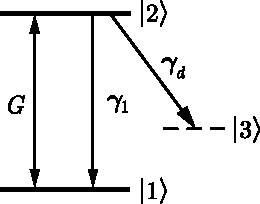
\includegraphics[width=4cm]{fig}
%  \caption{\label{f:fig}%
%  Подпись к рисунку.
%  }
%\end{figure}

%\begin{wrapfigure}{r}{0.35\textwidth}
%\centering
%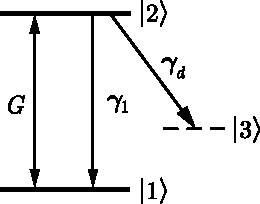
\includegraphics[width=4cm]{fig}
%\caption{\label{f:ff}%
%Рисунок <<в оборку>>.
%}
%\end{wrapfigure}

%Если разность энергий электронно-дырочных уровней $E_2 - E_1$ близка к энергии продольного оптического фонона $\hbar\Omega_{\mathrm{LO}}$, то в разложении волновых функций полного гамильтониана можно ограничиться нулевым приближением для всех состояний, за исключением близких по значению к $E_2$.
%Волновые функции последних представляют собой следующие комбинации вырожденных состояний\footnote{Текст сноски}.

%Ссылка на таблицу~\ref{t:InPSiO2}.
%\begin{table}[!ht]
%  \centering
%  \caption{Пример таблицы}\label{t:InPSiO2}
%  \begin{tabular}{l|ccc}
%    \hline\hline
%    & \quad$\lambda \cdot 10^{-11}$,~$\text{дин}\cdot\text{см}^{-2}$
%    & \quad$\mu \cdot 10^{-11}$,~$\text{дин}\cdot\text{см}^{-2}$
%    & \quad$\rho$, $\text{г}\cdot\text{см}^{-3}$ \\
%    \hline
%    InP       & 3.82 & 1.69 & 4.14 \\
%    SiO$_{2}$ & 1.57 & 3.11 & 2.2  \\
%    \hline\hline
%  \end{tabular}
%\end{table}

%\begin{figure}[!ht]
%  \centering
%  \begin{minipage}{5cm}
%    \centering
%    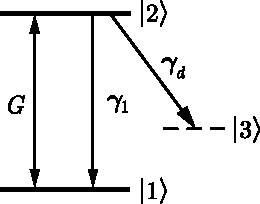
\includegraphics[width=4cm]{fig}
%    \caption{Рисунок с отдельным названием}
%  \end{minipage}
%  \quad
%  \begin{minipage}{5cm}
%    \centering
%    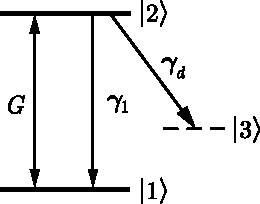
\includegraphics[width=4cm]{fig}
%    \caption{Рисунок с отдельным названием}
%  \end{minipage}
%  \quad
%  \begin{minipage}{5cm}
%    \centering
%    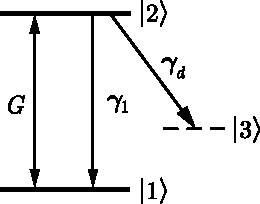
\includegraphics[width=4cm]{fig}
%    \caption{Рисунок с отдельным названием}
%  \end{minipage}
%\end{figure}

%\begin{figure}[!ht]
%  \centering
%  \begin{minipage}{5cm}
%    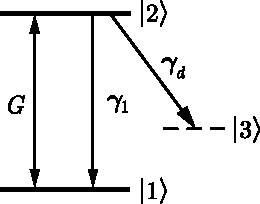
\includegraphics[width=4cm]{fig}
%  \end{minipage}
%  \begin{minipage}{5cm}
%    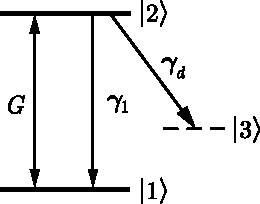
\includegraphics[width=4cm]{fig}
%  \end{minipage}
%  \caption{Рисунки с единым названием}
%\end{figure}

%Ссылка на внутренний рисунок (рис.~\ref{f:sub1}).

%\begin{figure}[!ht]
%\centering
%  \begin{minipage}{5cm}
%    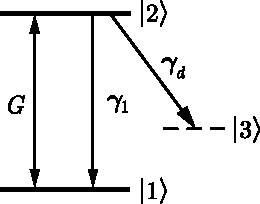
\includegraphics[width=4cm]{fig}\subcaption{}\label{f:sub1}
%  \end{minipage}
%  \begin{minipage}{5cm}
%    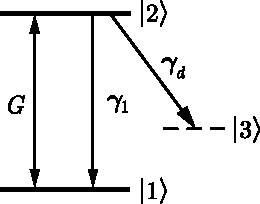
\includegraphics[width=4cm]{fig}\subcaption{}\label{f:sub2}
%  \end{minipage}
%  \begin{minipage}{5cm}
%    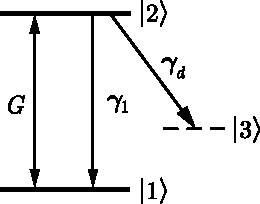
\includegraphics[width=4cm]{fig}\subcaption{}\label{f:sub3}
%  \end{minipage}
%  \caption[]{%
%  Рисунки с единым названием и подчиненной нумерацией:
%    \subref{f:sub1} ссылка 1,
%    \subref{f:sub2} ссылка 2,
%
%    \subref{f:sub3} ссылка 3.
%  }
%\end{figure}

%\subsection{Название подсекции}
%Текст подсекции
%\subsubsection{Название под-подсекции}
%Текст под-подсекции
%\paragraph{Название параграфа.}
%Текст параграфа
%\subparagraph{Название подпараграфа.}
%Текст подпараграфа

%Нумеруемый список:
%\begin{enumerate}
%  \item Первый уровень вложенности.
%  \begin{enumerate}
%    \item Второй уровень вложенности.
%    \begin{enumerate}
%      \item Третий уровень вложенности.
%    \end{enumerate}
%  \end{enumerate}
%\end{enumerate}

%Демонстрация полностью настраиваемых окружений типа <<теорема>>.

%\newtheorem{theorem}{Теорема}[chapter]
%\def\theoremstyle{}
%\def\postthetheorem{:}

%\newtheorem{lemm}{Лемма}[chapter]
%\def\thelemmstyle{\bfseries}
%\def\oparglemmstyle{}
%\def\lemmstyle{}
%\def\preoparglemm{(}
%\def\postoparglemm{):}

%\newtheorem{remark}{Примечание}[chapter]
%\def\remarkstyle{\itshape}
%\def\theremarkstyle{}
%\def\posttheremark{:}

%\begin{lemm}[Шура]
%Квадратная матрица, коммутирующая со всеми матрицами неприводимого представления, кратна единичной.
%\end{lemm}

%\begin{theorem}
%Гомоморфный образ группы изоморфен фактор-группе по ядру гомоморфизма.
%\end{theorem}

%\begin{remark}
%Текст примечания.
%\end{remark}
